%!TEX encoding = UTF-8 Unicode
% -*- coding: UTF-8; -*-
% vim: set fenc-utf-8

\chapter{Cas d'utilisations}
\label{s:cas_utilisation}

Ce chapitre présente les différents cas d'utilisation pour l'application VisuaLigue.
La figure \ref{fig:cas_utilisation_diag} résume les acteurs du systèmes et les cas d'utilisations.
La suite du chapitre décrie en détails les cas d'utilisations et s'attarde sur les plus importants.

\begin{figure}[htpb]
    \centering
    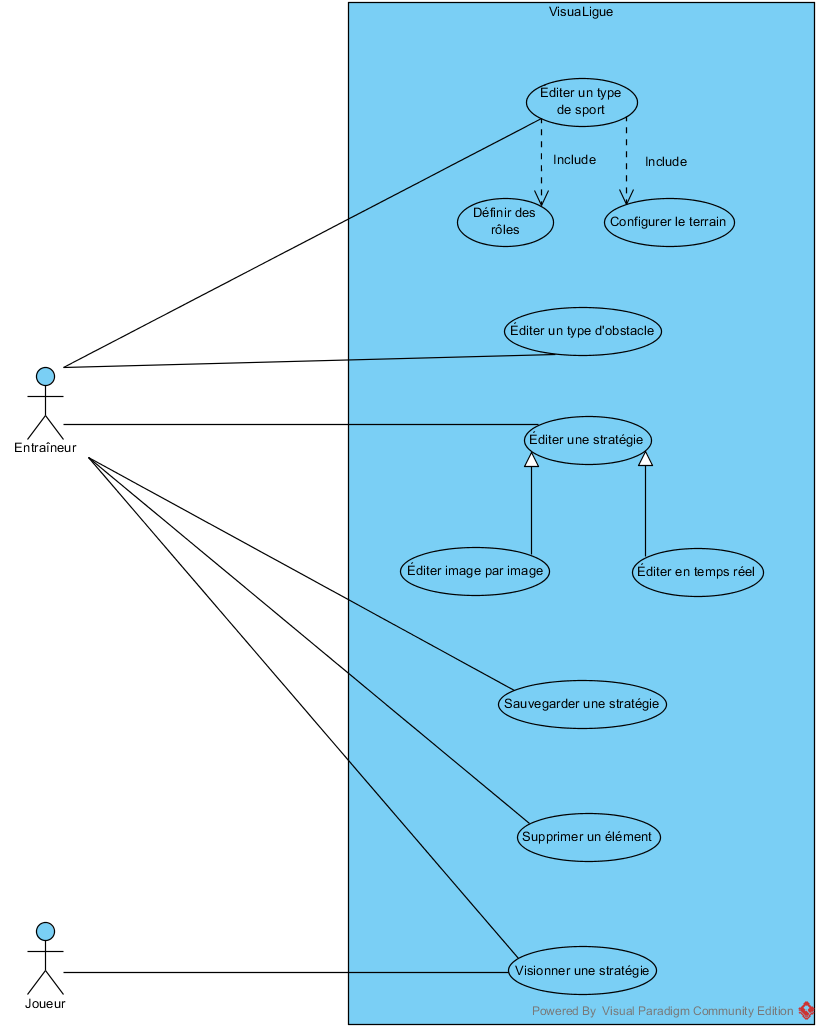
\includegraphics[scale=0.7]{fig/cas_utilisation_diag.png}
    \caption{Diagramme des cas d'utilisations}
    \label{fig:cas_utilisation_diag}
\end{figure}

\newpage



\section{Ajouter un type de sport}
\label{sec:ajouter_un_type_de_sport}

\begin{itemize}
    \item \textbf{Cas d'utilisation:} Ajouter un type de sport
    \item \textbf{Syst\`eme:} VisuaLigue
    \item \textbf{Acteur principal:} Entra\^ineur
    \item \textbf{Sc\'enario principal:}
        \begin{enumerate}
            \item L'entra\^ineur cr\'ee un sport, le nomme.
            \item Ensuite il ajoute les r\^oles du sport.
            \item Finalement, il d\'efini un terrain en dessinant les lignes et en sp\'ecifiant les dimensions.
        \end{enumerate}
    \item \textbf{Autres situations:}
    \begin{itemize}
        \item \textbf{Sport d\'ej\`a existant:} Si le sport existe d\'ej\`a dans l'application, un message d'avertissement appara\^it pour signaler que le sport existe d\'ej\`a.
        L'entraîneur peut d\'ecider d'effacer ce qui \'etait dans le sport existant, d'enregister son sport sous un autre nom, ou d'oublier le sport cr\'e\'e.
    \end{itemize}
\end{itemize}



\section{Ajouter une strat\'egie}
\label{sec:ajouter_une_strat'egie}
\begin{itemize}
    \item \textbf{Cas d'utilisation:} Ajouter une strat\'egie
    \item \textbf{Syst\`eme:} VisuaLigue
    \item \textbf{Acteur principal:} Entra\^ineur
    \item \textbf{Pr\'erequis:} Le sport pour lequel l'entraîneur veut ajouter une stratégie doit exister dans l'application.
    \item \textbf{Sc\'enario principal:}
        \begin{enumerate}
            \item L'entra\^ineur veut ajouter une nouvelle strat\'egie.
            \item Il lui assigne un identifiant et choisi un type de sport pour la strat\'egie.
        \end{enumerate}
    \item \textbf{Autres situations:}
        \begin{itemize}
            \item \textbf{Sport d\'ej\`a existant:}
            \begin{enumerate}
                \item Si la stratégie existe d\'ej\`a dans l'application, un message d'avertissement appara\^it.
                \item L'entra\^ineur a alors le choix entre \'ecraser la strat\'egie existante ou d'annuler son ajout.
            \end{enumerate}
        \end{itemize}
\end{itemize}



\section{\'Editer une stratégie}
\label{sec:ajouter_une_strategie}
\begin{itemize}
    \item \textbf{Cas d'utilisation:} \'Editer une strat\'egie
    \item \textbf{Syst\`eme:} VisuaLigue
    \item \textbf{Acteur principal:} Entra\^ineur
    \item \textbf{Pr\'erequis:} L'entraîneur a ajouté ou chargé une stratégie.
    \item \textbf{Parties prenantes et int\'er\^ets:}
    \item \textbf{Garanties en cas de succ\`es:}
    \item \textbf{Sc\'enario principal:}
        \begin{enumerate}
            \item L'entraîneur assigne les r\^oles aux diff\'erents joueurs.
            \item Ensuite, il peut s\'electionner un joueur et tracer un mouvement ou interargir avec le projectile.
            \item Pendant que le joueur est s\'electionn\'e, une simulation en temps r\'eel des mouvements pr\'ec\'edemment d\'efinies s'ex\'ecute.
            \item La simulation recommence du d\'ebut.
            \item L'entraîneur répète les étapes 2 et 4 pour chaque joueur jusqu'à ce que la stratégie soit terminé.
            \item L'entraîneur exécute \textit{sauvergarder une stratégie \ref{sec:exporter_une_strategie}}.
    \end{enumerate}
    \item \textbf{Autres situations:}
        \begin{itemize}
            \item \textbf{2a. Édition en mode image par image:} L'entraîneur édite la strat\'egie image par image ...
                \begin{enumerate}
                    \item L'entraîneur place les joueurs sur le terrain. 
                    \item L'entraîneur clique sur un boutton de l'application et avance d'une image. Les joueurs deviennent transparents.
                    \item L'entraîneur clique sur un joueur et le glisse vers sa nouvelle position.
                    Le joueur sélectionné n'est plus transparent.
                    \item L'entraîneur répète l'étape 3 pour tous les joueurs qu'il veut déplacer.
                    \item L'entraîneur répète les étapes 2 à 4 jusqu'à ce qu'il ait terminé sa stratégie. 
                    \item L'entraîneur continue le scénario principal à partir de l'étape 6.
                \end{enumerate}
            \item \textbf{*a. visualiser la stratégie}
            À tout moment de l'édition de la stratégie. l'entraîneur peut exécuter \textit{visualiser la stratégie}.
 
        \end{itemize}
    \item \textbf{Fr\'equence d'utilisation:}
\end{itemize}



\section{Visualiser une stratégie}
\label{sec:visualiser_une_strategie}
\begin{itemize}
    \item \textbf{Cas d'utilisation:} Visualiser une strat\'egie
    \item \textbf{Syst\`eme:} VisuaLigue
    \item \textbf{Acteur principal:} Entra\^ineur ou joueur
    \item \textbf{Parties prenantes et int\'er\^ets:}
    \item \textbf{Pr\'erequis:} Il faut que la strat\'egie soit enregistr\'ee dans l'application pour que l'entraîneur puisse la visualiser.
    \item \textbf{Garanties en cas de succ\`es:}
    \item \textbf{Sc\'enario principal:}
        \begin{enumerate}
            \item L'entra\^ineur s\'electionne la strat\'egie \`a visualiser.
            \item Il d\'ebute la visualisation et observe le d\'eroulement de la strat\'egie.
            \item Il peut mettre fin \`a la visualisation \`a tout moment.
        \end{enumerate}
    \item \textbf{Autres situations:}
        \begin{itemize}
            \item fubar
                \begin{enumerate}
                    \item foo
                    \item bar
                \end{enumerate}
        \end{itemize}
\end{itemize}



\section{Sauvegarder une stratégie}
\label{sec:exporter_une_strategie}
\begin{itemize}
    \item \textbf{Cas d'utilisation:} Sauvegarder une strat\'egie
    \item \textbf{Syst\`eme:} VisuaLigue
    \item \textbf{Acteur principal:} Entra\^ineur
    \item \textbf{Sc\'enario principal:}
        \begin{enumerate}
            \item L'entra\^ineur a modifié une strat\'egie et la sauvegarde.
            \item L'application enregistre les \'el\'ements de la strat\'egie.
        \end{enumerate}
    \item \textbf{Autres situations:}
        \begin{itemize}
            \item \textbf{Exportation dans un format d'image:}
                \begin{enumerate}
                    \item L'entra\^ineur souhaite plut\^ot exporter la strat\'egie dans un format de fichier.
                    \item Il s\'electionne le format de fichier et le nom pour l'exportation.
                    \item L'application convertie la strat\'egie en une image et l'enregistre dans un fichier avec le bon nom.
                \end{enumerate}
        \end{itemize}
\end{itemize}



\section{Charger une strat\'egie}
\label{sec:charger_une_strat'egie}

\begin{itemize}
    \item \textbf{Cas d'utilisation:} Charger une strat\'egie
    \item \textbf{Syst\`eme:} VisuaLigue
    \item \textbf{Acteur principal:} Entra\^ineur
    \item \textbf{S\'ecnario principal:}
        \begin{enumerate}
            \item L'entra\^ineur souhaite \'editer une strat\'egie d\'ej\`a existante.
            \item Il s\'electionne la bonne strat\'egie puis la charge.
        \end{enumerate}
\end{itemize}
